\documentclass[12pt,fleqn]{article}\usepackage{../common}
\begin{document}
%sf. 112
%Janert 238 oku, 

Ders 5

Guven Araligi (Confidence Intervals)

Bu kavram istatistikte tartisilan konulardan biri. Bayes ve Frenkans�� 
(Frequentist) istatistik arasindaki felsefi farklardan biri burada ortaya
cikiyor. Frekansci tanim soyledir:

\begin{quote}
Bir parametre $\theta$ icin $1-\alpha$ seviyesinde bir $C_n=(a,b)$ guven araligi
tanimlanabilir -- bu aralik $a=a(X_1,..,X_n)$ ve $b=b(X_1,..,X_n)$ adli iki
fonksiyon uzerinden tanimlanabilir. Bu fonksiyonlar veri uzerinde isleyen, 
{\em verinin} fonksiyonlaridir, ve sonucta

\[ \mathbb{P}_\theta (\theta \in C_n) \ge 1-\alpha, \ \ \forall \theta \in \Theta \]

Yani $(a,b)$ araligi $1-\alpha$ olasiliginda $\theta$'yi icine alir /
hapseder. Daha detayli olarak deney arka arkaya pek cok kez
tekrarlandiginda parametrenin tahmininin $1-\alpha$ oraninda tanimlanan
araliga dusecegi soylenir. $1-\alpha$ sayisina guven araliginin kapsami
(coverage) ismi de verilir. Genellikle insanlar yuzde 95 guven araligini
kullanirlar, ve bu yuzdeye tekabul eden $\alpha = 0.05$ rakami kullanilir.

Uzerine basarak belirtmek gerekir ki $C_n$ rasgele (random) bir degerdir,
ama $\theta$ sabittir, cunku $C_n$ verinin bir fonksiyonudur, ve veriden,
yani bir orneklemden gelecegi icin o da rasgele olmalidir.

Eger $\theta$ bir vektor ise o zaman bir aralik yerine bir guven kumesi
kullanilir (mesela bir kure, ya da elips). 
\end{quote}

Fakat frekansci yaklasimda aralik fonksiyonlari $a,b$ ile guven araligi
arasindaki baglanti net degildir. Hangi fonksiyon secimi hangi $\alpha$'ya
sebebiye vermektedir? Bu durum net oldugu durumlarda bile teorik olarak
saglamligi suphelidir, ayrica hesabin sozel olarak ortaya konmasinda bazi
eksikler vardir. ``Deney arka arkaya pek cok kez tekrarlandiginda
parametrenin tahmini, $1-\alpha$ guven araliga dusecektir'' ibaresi
mesela; ``deney tekrari'' her durumda gecerli olmayabilir. Meteoroloji
``yarin yuzde 80 ihtimali ile yagmur yagacak'' diyorsa, o hesap sartlarinin
bir daha ortaya cikmasinin olasiligi cok dusuktur, Kaos Teorisi bize en
azindan bunu soyluyor.

Wiki sayfasinda [1] tartismanin boyutlari gorulebilir.

Son onyillarda ortaya cikan yaklasim ise Bayes Teorisini devreye
sokmak. Bir guven araligi tanimlamanin en saglam yolu bu hesabi tek bir
dagilim uzerinde yapmak. Eger sonuc olarak bir tekil sayi degil, bir
dagilim elde edersek bu dagilim uzerinde guvenlik hesaplarini yapmak cok
kolay hale gelir. Mesela sonuc bir Gaussian dagilim ise, bu dagilimin yuzde
95 agirliginin nerede oldugu, ve nasil hesaplandigi bellidir.

Bayes Teorisi

\[ P(A|B)  = \frac{ P(B|A)P(A)}{P(B)} \]

Veri analizi baglaminda diyelim ki deneyler yaparak tahmini olarak
hesaplamak (estimate) istedigimiz bir parametre var, bu bir protonun
kutlesi ya da bir ameliyat sonrasi hayatta kalma orani olabilir. Bu
durumlarda iki ayri ``olaydan'' bahsetmemiz gerekir, B olayi spesifik bazi
olcumlerin elde edilmesi ``olayidir'', mesela olcum uc sayidan olusuyorsa,
biz bir olcumde spesifik olarak $\{0.2,4,5.4\}$ degerlerini elde
etmisiz. Ikinci olay bilmedigimiz parametrenin belli bir degere sahip
olmasi olacak. O zaman Bayes Teorisinin su sekilde tekrar yazabiliriz, 

\[ P(parametre | veri ) \propto P(data | parametre)P(parametre) \]

$\propto$ isareti orantili olmak (proportional to) anlamina geliyor. Boleni
attik cunku o bir sabit (tamamen veriye bagli, tahmini hesaplamak
istedigimiz parametreye bagli degil). Tabii bu durumda sol ve sag taraf
birbirine esit olmaz, o yuzden esitlik yerine orantili olmak isaretini
kullandik. Bu cercevede ``belli bir numerik sabit cercevesinde birbirine
esit (equal within a numeric constant)'' gibi cumleler de gorulebilir. 

Ornek

Diyelim ki bir bozuk para ile 10 kere yazi-tura attik, ve sonuc altta

T H H H H T T H H H

Bu veriye bakarak paranin hileli olup olmadigini anlamaya
calisacagiz. Bayes ifadesini bu veriye gore yazalim,

\[ P(p | \{ \textrm{T H H H H T T H H H} \} \propto 
P(\{ \textrm{T H H H H T T H H H} | p) P(p) \}
\]

$P(p)$ ifadesi ne anlama gelir? Aslinda bu ifadeyi $P([Dagilim] = p)$
olarak gormek daha iyi, artik $p$ parametresini bir dagilimdan gelen bir
tekil deger olarak gordugumuze gore, o dagilimin belli bir $p$'ye esit
oldugu zamani modelliyoruz burada. Her halukarda $P(p)$ dagilimini, yani
onsel (prior) olasiligi bilmiyoruz, hesaptan once her degerin mumkun
oldugunu biliyoruz, o zaman bu onsel dagilimi duz (flat) olarak aliriz,
yani $P(p) = 1$. 

$P(\{\textrm{T H H H H T T H H H} | p)$ ifadesi goz korkutucu olabilir, ama
buradaki her ogenin bagimsiz ozdesce dagilmis (independent identically
distributed) oldugunu gorursek, ama bu ifadeyi ayri ayri
$P(\{\textrm{T}|p)$ ve $P(\{\textrm{H}|p)$ carpimlari olarak gorebiliriz. $P(\{\textrm{T}|p) = p$ ve 
$P(\{\textrm{H}|p)=1-p$ oldugunu biliyoruz. O zaman 

\[ P(p | \{ \textrm{7 Tura, 3 Yazi} \} \propto
p^7(1-p)^3
\]

Grafiklersek, 

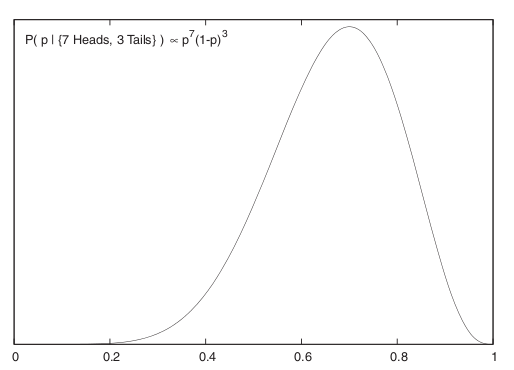
\includegraphics[height=8cm]{05_01.png}

Boylece $p$ icin bir sonsal (posterior) dagilim elde ettik. Artik bu
dagilimin yuzde 95 agirliginin nerede oldugunu rahatca gorebiliriz /
hesaplayabiliriz. Dagilimin tepe noktasinin $p=0.7$ civarinda oldugu
goruluyor. Bir dagilimla daha fazlasini yapmak ta mumkun, mesela bu
fonksiyonu $p$'ye bagli baska bir fonksiyona karsi entegre etmek mumkun,
mesela beklentiyi bu sekilde hesaplayabiliriz. 










Kaynaklar

[1] http://en.wikipedia.org/wiki/Confidence\_interval

\end{document}
